\section{Thursday, March 6: Fitting a neural network: backpropagation and gradient descent}

Recall from Monday that our neural network model with one hidden later is a model that makes predictions of the form:
\begin{equation}
\label{nn_thurs}
\hat{y} = f(X) = \beta_0 + \sum_{k=1}^K \beta_k g\left(w_{k0}+\sum_{j=1}^p w_{kj} x_j\right). 
\end{equation}
Because this is a lot of parameters to keep track of, we sometimes draw the model as a picture. But ultimately, given our neural network architecture (our picture, which should tell us $K$ and should tell us if the network is ``fully connected"), we need to use our training data to FIT the network.

This just means coming up with values $\hat{\theta} = (\hat{w}_{01}, \ldots, \hat{w}_{Kp}, \hat{\beta}_0, \ldots, \hat{\beta}_K)$ that minimize the error over our training set: 
$$
\sum_{i=1}^n (Y_i - \hat{Y}_i)^2.
$$
Of course eventually we will also care about overfitting and test error. But to start, let's just figure out how we might even minimize the loss when $\hat{Y}_i$ has the form in \eqref{nn_thurs}. It is not going to be simple! We are going to need to use an optimization technique called gradient descent. The key insight for neural networks is that we can use the chain rule to do gradient descent in a very organized way, called backpropagation. 

\subsection{Gradient descent}

Let $\theta$ be a long vector that stores all of our parameters in our network. So our goal is to minimize, with respect to $\theta$, 
$$
L(\theta) = \sum_{i=1}^n (Y_i - \hat{Y}_i)^2.
$$
Unfortunately, for neural networks, this is too complicated to just take the derivative with respect to every single parameter and set them equal to $0$. This would be a massive system of equations.

So instead of solving for a minimum directly, let's try to do it iteratively.

Let's start with $\theta^{0}$: a set of random guesses for every parameter in the network. These values will produce estimates $|hat{Y}_i$ for every element in our training set: they probably will just not be very good estimates!

Then, let's take steps along the negative gradient (with respect to $\theta$) of the loss function. The gradient of $L(\theta)$ with respect to $\theta$ is denoted $\nabla L(\cdot)$. The gradient is simply the vector of partial derivatives with respect to each element of $\theta$.  Once we have taken this step, we will update our values of all of our parameters, so $\theta^{0}$ becomes $\theta^{1}$. This new vector then yields new predictions $\hat{Y}$ for every training point.

The idea is that, if we take steps in the direction of the negative gradient of the loss function, we always move a current guess $\theta^t$ to a new guess $\theta^{t+1}$ in a way that will make the loss smaller the next time we compute it. What a nice idea!

While we take a step in the ``direction" of the gradient, we don't want to take a step that is the SIZE of the gradient. We want to take really small steps so that we don't ``overshoot" a minimum. So we let: 
$$
\theta^{t+1} = \theta^t - \rho \nabla L(\theta^{t}),
$$
where $\rho$ is a small learning rate that we get to pick. Picking it can actually be really finicky: if it is TOO small you will never find a good value of $\theta$. But if it is too big you can ``overshoot" a minimum. 

Note: if our step size $\rho$ is going to be approximately the same for all elements of $\theta$, we probably want the elements of $\theta$ to all be in the same ``units". This means that we probably want to normalize our input variables $X$! This is not changed from other algorithms. 

We keep taking small steps in the direction of the negative gradient until our ``guesses" stop changing. At this point, we have landed in a region of $\theta$-space where the derivative is 0! This hopefully means that we found a minimum of the loss function!

Unfortunately, there is no guarantee that it is a global minimum. For really complicated non-convex loss functions, we can get stuck in suboptimal local minima. We will discuss strategies for avoid it later! For now, see Figure~\ref{fig_gd} for an illustration of gradient descent in a setting where $\theta$ is one-dimensional. 

Gradient descent is a really general optimization technique! It is used in contexts that have nothing to do with fitting neural networks!

\begin{figure}[h]
\centering 
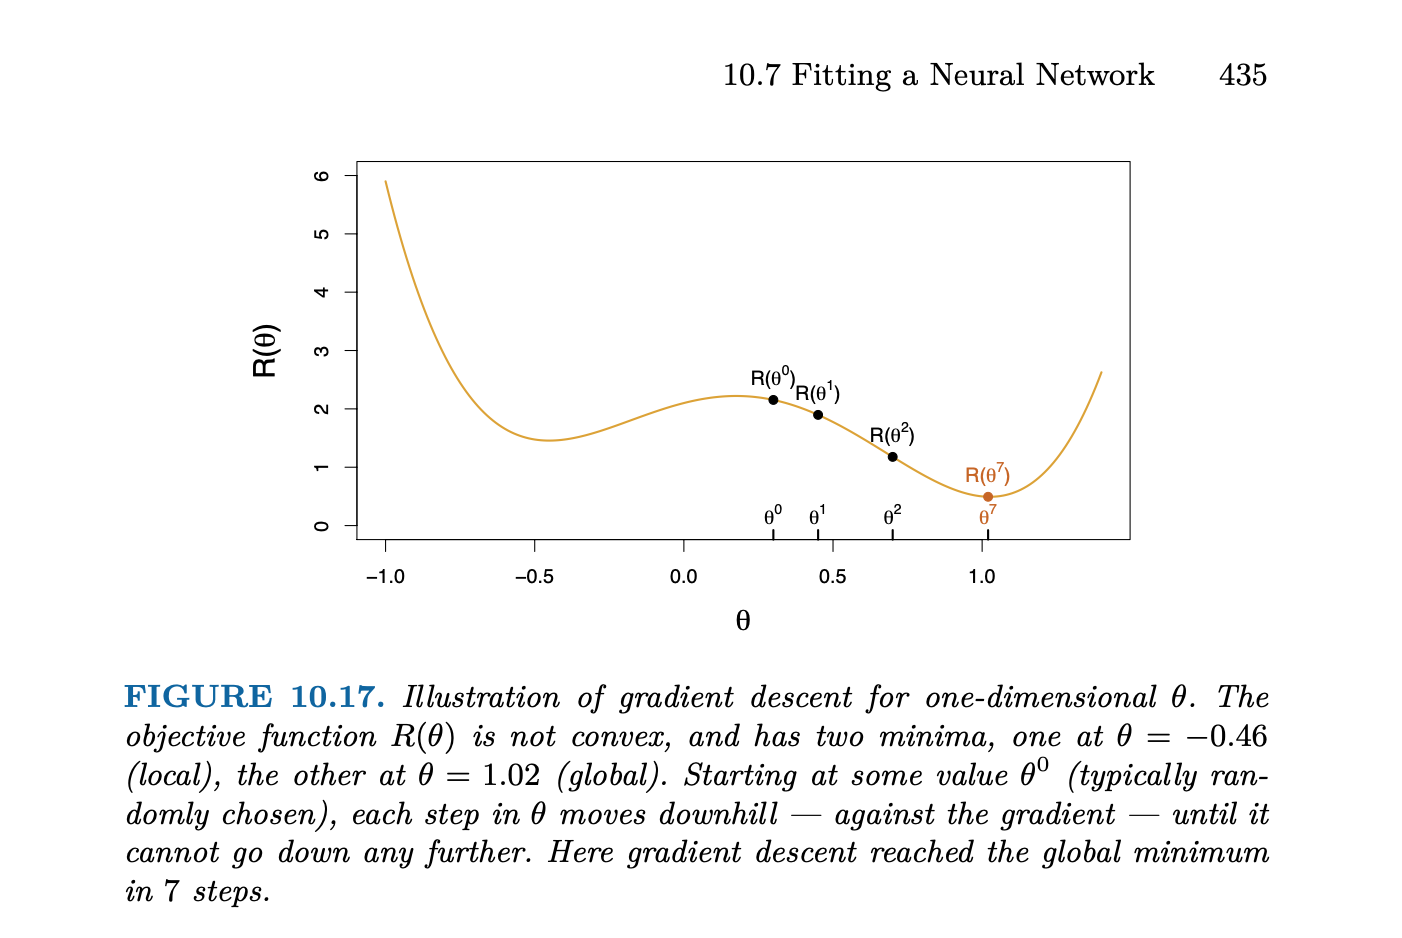
\includegraphics[width=0.7\textwidth]{442_lecs/gradient.png}
\caption{An illustration from ISL of gradient descent for a very simple one-dimensional $\theta$. In this case, we found the global minimum. But that is not guaranteed!}
\label{fig_gd}
\end{figure}

\subsection{Backpropagation and the Chain Rule}

Let's study gradient descent for a one-layer feed-forward neural network in the following very simple case. This is a network with one hidden later and three hidden nodes ($K=3)$. There are also only three inputs ($p=3$). For simplicity, I did not draw the intercept (bias) terms only the diagram.

\begin{center}
\begin{tikzpicture}[
    node distance=1.5cm and 2.5cm,
    neuron/.style={circle, draw, minimum size=1cm},
    every label/.style={font=\small}
]

% Input layer
\node[neuron, fill=yellow!50] (I1) {$x_1$};
\node[neuron, fill=yellow!50, below=of I1] (I2) {$x_2$};
\node[neuron, fill=yellow!50, below=of I2] (I3) {$x_3$};

% Hidden layer
\node[neuron, fill=cyan!30, right=of I1, label=above:\textcolor{blue}{$A_1$}] (H1) {$g(w_1^T x)$};
\node[neuron, fill=cyan!30, right=of I2, label=above:\textcolor{blue}{$A_2$}] (H2) {$g(w_2^T x)$};
\node[neuron, fill=cyan!30, right=of I3, label=above:\textcolor{blue}{$A_3$}] (H3) {$g(w_3^T x)$};

% Output layer
\node[neuron, fill=purple!50, right=of H2, label=above:\textcolor{purple}{$\hat{y}$}] (O) {$f(\beta_0 + \beta^T A)$};

% Connections (Input to Hidden)
\foreach \i in {I1, I2, I3}
    \foreach \h in {H1, H2, H3}
        \draw[->] (\i) -- (\h);

% Connections (Hidden to Output)
\foreach \h in {H1, H2, H3}
    \draw[->] (\h) -- (O);

% Label the specific weights
\draw[->] (I1) -- node[above] {\small $w_{11}$} (H1);
\draw[->] (I3) -- node[above] {\small $w_{31}$} (H3);
\draw[->] (H1) -- node[above] {\small $\beta_1$} (O);
\draw[->] (H2) -- node[above] {\small $\beta_2$} (O);
\draw[->] (H3) -- node[above] {\small $\beta_3$} (O);
\end{tikzpicture}
\end{center}

In this case, suppose that we are doing regression, and so the function $f()$ at the very end is just the identity function. Recall that when we are doing classification, we need to turn our final output into a probability or a prediction using a link function. But for regression we are all set on our original scale. 

For given values of $w_{10},\ldots, w_{pK}$ and $\beta_0,\ldots, \beta_K$, each input example $x_i$ gets turned into a $\hat{y}_i$. Our squared error loss for our training set is: 
\begin{align*}
L(\theta) &= \sum_{i=1}^n L_i(\theta) = \sum_{i=1}^n (y_i - \hat{y}_i)^2 \\
&= \sum_{i=1}^n \left( y_i - \beta_0 - \sum_{k=1}^3 \beta_k A_k \right)^2 \\
&= \sum_{i=1}^n \left( y_i - \beta_0 - \sum_{k=1}^3 \beta_k g \left(w_{k0} + \sum_{j=1}^p w_{kj} x_{ij}\right)\right)^2. 
\end{align*}

I wrote this at multiple levels of granularity. Sometimes it is nice to explicitly see that the loss function depends on every $w$ and every $\beta$. Other times, it is kind of nice to hide this detail. 

Suppose that we begin with random guesses for every $\beta$ and every $w$. Then, we send our entire training set ``forward" through the neural network and compute this loss function given the current predictions. Then, we compute the gradient. We step along the gradient, and we update our guesses of $w$ and $\beta$ accordingly. 

For our neural network loss function, let's figure out the steps along the gradient. The key idea is that we can chain rule! 

In this example, since $f()$ is just the identity function, we have that:
\begin{align*}
\frac{dL}{d \beta_k} &= -2 \sum_{i=1}^n (y_i - \hat{y}_i) \frac{d\hat{y}_i}{d \beta_k} \\
&= - 2 \sum_{i=1}^n (y_i - \hat{y}_i) A_k \\
&= -2 \sum_{i=1}^n (y_i - \hat{y}_i) g \left(w_{k0} + \sum_{j=1}^p w_{kj} x_{ij}\right) 
\end{align*}
And then:
\begin{align*}
\frac{dL}{d w_{kj}} &= -2 \sum_{i=1}^n (y_i - \hat{y}_i) \frac{d\hat{y}_i}{d w_{kj}} \\
&= -2 \sum_{i=1}^n (y_i - \hat{y}_i ) \beta_{k} g' \left(w_{k0} + \sum_{j=1}^p w_{kj} x_{ij}\right) x_{ij},
\end{align*}
where the specific form depends on the activation function $g()$. But hopefully we choose a differentiable $g()$ where this isn't too complicated.

Note that both of these partial derivatives imply that the direction of our step depends on our residuals $y_i - \hat{y}_i$: this is a good thing! We want to make the residuals smaller! 

The reason that we call this special version of gradient descent ``backpropagation" is that we can think of these applications of the chain rule as stepping backward through our network, and passing our residuals/errors along as we go. As we add more layers to the network, we add more chain rules! But nothing gets too difficult. 

Recall that gradient descent lets:
$$
\theta^{t+1} = \theta^t - \rho \nabla L (\theta^{t}).
$$
So, the size of the step depends on the learning rate $\rho$, the size of the residuals $(y_i - \hat{y}_i)$, the magnitude of the gradient evaluated at $\theta^{t}$, and the actual inputs $x_{ij}$. This is a lot of things! Making sure that we take the right sized steps can be very finicky. 

\subsection{Stochastic Gradient Descent}

Instead of computing the loss function and the gradient over all $n$ training instances at once, we typically go instance-by-instance or batch-by-batch. This is related to \emph{online learning}, which you read about for HW2. A batch is just a subset of the $n$ training observations. The motivation is that we will speed up our learning about $\theta$ by updating $\theta^{t}$ more often. If our training set is huge, we don't want to bother processing a massive training set with a bad guess $\theta^{t}$. We should take advantage of the fact that we see a lot of errors in the first few training examples, and we should update $\theta^{t}$ to $\theta^{t+1}$ right away. 

If we are using SGD and we end up iterating through the entire training set 10 times, this means that we used 10 epochs. But, this might mean that we used $T=100$ updates of $\theta$, if our batch size was 1/10 of the training set. We need to decide how many epochs we want, etc. 

This is stochastic because our gradient computed on a small number of training observations should be a good approximation of our overall gradient. But the exact step we take depends on the specific training observation! It also turns out that the extra noise added with SGD can help us avoid local minima! That is cool too! We bounce around $\theta$-space and explore a bit more. 

Very strangely: it turns out that stochastic gradient descent enforces its own form of approximately quadratic regularization. I don't think that this is at all obvious. I learned from preparing for this class that the reason is because stochastic gradient descent gives updates for $\theta$ that remain in the row space of the inputs. Out of all solutions that would give $0$ training error (in a setting where this is possible), stochastic gradient descent is supposed to find the one with the smallest L2 norm. ``Supposed to" because I think it still might not due to initial conditions and step size. But anyway, I don't think this was the motivation for people coming up with SGD, but it is a recently studied property, and it explains double descent!! So cool. 





\subsection{Complications}

While (stochastic) gradient descent is a very general idea that can be used in many contexts, it is ultimately only a way to find an approximate minimizer of a loss function. There are a lot of complications.
\begin{itemize}
\item We need to choose good initial guesses for the parameters. If we choose bad ones, we can get stuck at local minima.
\item We need to choose a good step size! To converge in a reasonable about of time without jumping over minima. 
\item We have to worry about ``vanishing gradients" / the dead ReLU: where once a ReLU unit is outputting a 0 for every training example, its weights never get updated again. 
\item We need to choose batch size for SGD.
\item We need to choose how many iterations or epochs to train for. In theory, I guess we should go until the $\theta^t$ stop changing (convergence). But ... what if we have used up all of our computational resources and we have not yet converged? 
\item We also need to pick our model architecture! How many hidden nodes do we want? How many hidden layers? What activation function should we use? 
\end{itemize}

Previously, to pick a tuning parameter, you used cross validation. Doing cross validation for ALL of these choices and coming up with the best possible parameter sets is a full time job. And, literally, this is a full time job that you could all go get! TLDR: you basically need to be an expert to fit a neural network. It is not an ``off-the-shelf" algorithm. 


\subsection{Overfitting and model complexity}

We know that a neural network model with $K$ hidden units in one layer and $p$ inputs needs to learn around $(p+1)*(K+1)$ parameters. If we add more hidden laters, this just gets bigger.

We know that, if we have $n$ training datapoints, a model with more than $n$ parameters should be able to memorize the training set. And we know that this is bad, because we will overfit, and will have poor generalization error. 

In modern deep neural networks, we often have more parameters than datapoints! So, how can we prevent overfitting?

There are several strategies that people were already doing:
\begin{itemize}
\item Add explicit regularization to our loss function! Like $\lambda$ times the L1 or L2 norm of our $w$s and our $\beta$s. This affects every step of our gradient descent calculation, and could make it more complicated. But it will keep the variance of our model down, as we know. 
\item Random dropout: A possibly simpler version of regularization. We can just randomly turn off some hidden nodes when we pass some training observations through the network. This forces other nodes to pick up the slack of these turned-off nodes. This means that a single node cannot be used to memorize a single training point---- because it has to perform multiple tasks. What a super cool idea!  
\item Early stopping via a validation set. Suppose that we want to encourage our weights to be small. We can start with small initial values. Then, every time we finish a batch or an epoch, we can check our error on a validation set. Presumably at first, this will be decreasing as we update our weights. If, at some point it starts increasing, we can assume that we started overfitting, and we can just stop training (even if we haven't converged). This is cool and should also work well! 
\end{itemize}
Note that any type of regularization adds to our training complications. How to we pick our penalty parameter? How do we pick how much dropout to have, or how MUCH the validation error needs to increase in order for us to think we should stop? There is already so much going on! This is not automated! 

Ok, but even with all of these strategies, don't we think that these massive models will overfit? And perform badly in terms of the bias-variance tradeoff? Especially when we don't have that many training observations? 
\begin{itemize}
\item Mostly, yes I do think this!
\item But empirically, we have seen a strange phenomenon called double descent.
\item It turns out it is not actually that strange or mysterious! Let's explore. 	
\end{itemize}


\subsection{Double descent, and its relation to stochastic gradient descent}

This is one of my favorite topics! See ISL 10.8 for a beautiful explanation. You will also explore this concept on your homework, and I may fill in these notes in more detail after Thursday's class. 

The story of double descent is shown in Figure~\ref{fig_dd}. We know that as the degrees of freedom in a model approaches $n$, the training set size, the training error goes to $0$. This is the interpolation threshold; or the point at which our model is simply memorizing the training data.

Classical statistical theory says that the test set should be really bad at this point.

But, in practice, people noticed that for deep learning, you could keep making the model MORE complex (more layers, more nodes) AFTER the interpolation threshold, and while the training error remains 0, the test error starts to decrease again. This is called double descent: and some people thought it was magic! They thought it totally changed our interpretation of ALL of statistics!! What happened to the bias-variance tradeoff?

It turns out that the issue with this plot is what we draw on the X-axis. If we draw the X-axis as ``number of parameters", double descent does indeed happen. But if we correctly make the axis the degrees of freedom, we will not see the double descent phenomenon. See this awesome recent paper: \url{https://proceedings.neurips.cc/paper_files/paper/2023/hash/aec5e2847c5ae90f939ab786774856cc-Abstract-Conference.html}. 

On your homework, you will see how this plays out for linear regression onto natural splines. It turns out that, if we continue to increase the degrees of freedom of our spline basis past the interpolation threshold, we end up doing some automatic regularization that we didn't (necessarily) realize we were doing. This means that we aren't actually just increasing model complexity without bound! We are fitting a regularized model, and so number of parameters is no longer equal to model complexity. 

For deep learning, it turns out that stochastic gradient descent actually does implicit regularization. If there are many possible parameter vectors that would all give the same interpolating solution, SGD finds the minimum-norm solution. This is regularization! So ... there is no magic. Deep learning performs well because it has no bias and is ALSO regularized to have low variance. 

\begin{figure}
\centering 
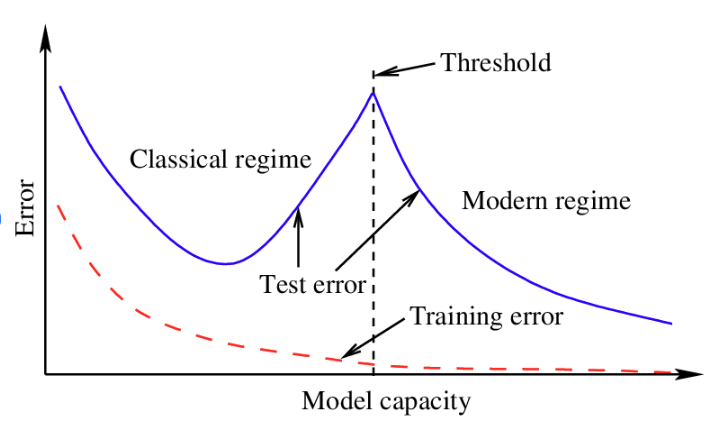
\includegraphics[width=0.6\textwidth]{442_lecs/dd.png}
\caption{A classic illustration of double descent.}	
\label{fig_dd}
\end{figure}


\subsection{Extensions of neural networks}

We have barely scratched the surface. There are so many cool topics we could cover. Such as multitask learning, auto-encoders, convolutional neural networks, or recurrent neural networks. Auto-encoders also relate to semi-supervised learning. We are not going to cover these! But hopefully you now have a little bit of foundational knowledge to understand these better in the future. And you could always do one of these for your final project!




